\documentclass[tikz]{standalone}
\usepackage{cancel}
\usepackage{fontspec}
\setmonofont[Scale=MatchLowercase]{DejaVu Sans Mono}
\usetikzlibrary{arrows.meta}

\begin{document}
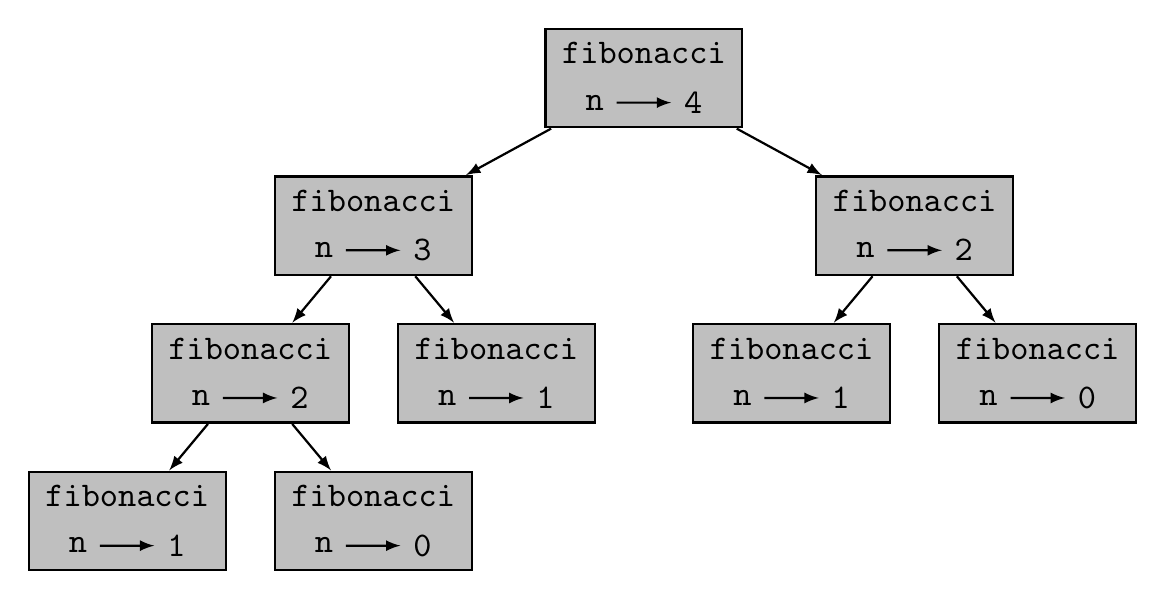
\begin{tikzpicture}[thick, scale=1.25, transform shape]
$\node(fib4) [draw, fill=lightgray, minimum width=2cm, minimum height=1cm]{};
\node at (0,0.25){\tt fibonacci};
\node(f4n) at (-0.5, -0.25){\tt n};
\node(f4) at (0.5, -0.25){\tt 4};
\draw[-latex] (f4n)--(f4);
\node(fib3) [draw, fill=lightgray, minimum width=2cm, minimum height=1cm] at(-2.75,-1.5){};
\node at (-2.75,-1.25){\tt fibonacci};
\node(f3n) at (-3.25, -1.75){\tt n};
\node(f3) at (-2.25, -1.75){\tt 3};
\draw[-latex] (f3n)--(f3);
\node(fib2) [draw, fill=lightgray, minimum width=2cm, minimum height=1cm] at(2.75,-1.5){};
\node at (2.75,-1.25){\tt fibonacci};
\node(f2n) at (2.25, -1.75){\tt n};
\node(f2) at (3.25, -1.75){\tt 2};
\draw[-latex] (f2n)--(f2);
\node(fib22) [draw, fill=lightgray, minimum width=2cm, minimum height=1cm] at(-4,-3){};
\node at (-4,-2.75){\tt fibonacci};
\node(f22n) at (-4.5, -3.25){\tt n};
\node(f22) at (-3.5, -3.25){\tt 2};
\draw[-latex] (f22n)--(f22);
\node(fib1) [draw, fill=lightgray, minimum width=2cm, minimum height=1cm] at(-1.5,-3){};
\node at (-1.5,-2.75){\tt fibonacci};
\node(f1n) at (-2, -3.25){\tt n};
\node(f1) at (-1, -3.25){\tt 1};
\draw[-latex] (f1n)--(f1);
\node(fib11) [draw, fill=lightgray, minimum width=2cm, minimum height=1cm] at(1.5,-3){};
\node at (1.5,-2.75){\tt fibonacci};
\node(f11n) at (1, -3.25){\tt n};
\node(f11) at (2, -3.25){\tt 1};
\draw[-latex] (f11n)--(f11);
\node(fib0) [draw, fill=lightgray, minimum width=2cm, minimum height=1cm] at(4,-3){};
\node at (4,-2.75){\tt fibonacci};
\node(f0n) at (3.5, -3.25){\tt n};
\node(f0) at (4.5, -3.25){\tt 0};
\draw[-latex] (f0n)--(f0);
\node(fib111) [draw, fill=lightgray, minimum width=2cm, minimum height=1cm] at(-5.25,-4.5){};
\node at (-5.25,-4.25){\tt fibonacci};
\node(f111n) at (-5.75, -4.75){\tt n};
\node(f111) at (-4.75, -4.75){\tt 1};
\draw[-latex] (f111n)--(f111);
\node(fib00) [draw, fill=lightgray, minimum width=2cm, minimum height=1cm] at(-2.75,-4.5){};
\node at (-2.75,-4.25){\tt fibonacci};
\node(f00n) at (-3.25, -4.75){\tt n};
\node(f00) at (-2.25, -4.75){\tt 0};
\draw[-latex] (f00n)--(f00);
\draw[-latex] (fib4)--(fib3);
\draw[-latex] (fib4)--(fib2);
\draw[-latex] (fib3)--(fib22);
\draw[-latex] (fib3)--(fib1);
\draw[-latex] (fib2)--(fib11);
\draw[-latex] (fib2)--(fib0);
\draw[-latex] (fib22)--(fib111);
\draw[-latex] (fib22)--(fib00);
$
\end{tikzpicture}
\end{document}
